\section{Implementazione e Funzionamento}

\subsection{Server}

Analizziamo come prima cosa il funzionamento dell'intero server andando poi a focalizzare l'attenzione sugli aspetti implementativi pi\`u importanti.
Il main della parte server dell'applicazione si trova nella classe BitCreekServer all'interno del package $server$, all'avvio viene istanziato un nuovo oggetto BitCreekServer e contestualmente alla sua creazione (quindi nel costruttore) viene ripristinato uno stato consistente a partire da un file di configurazione. Successivamente vengono avviati i thread ServerListener e ThreadSaver ed infine avviato RMI.
Si noti che le porte utilizzate come ServerSocket per la connessione dei peer e come porta RMI sono fissate a programma questo perch\'e abbiamo ritenuto che un server abbia piena disponibilit\`a delle proprie porte, diversamente nel lato client abbiamo creato un complesso sistema di gestione del NAT interattivo e a runtime per la scelta delle porte.
Nel file di configurazione viene salvato lo stato di ogni swarm di cui il server tiene traccia, al momento della creazione del server vengono ripristinati (per ogni swarm) tre thread, un thread tracker di keepalive su UDP, un thread tracker per gestire i nuovi peer che si aggiungono allo swarm e infine un thread Trimmer.
Il thread ServerListener si occupa di gestire le richieste di connessione al server da parte dei peer e fornisce meccanismi per la gestione del NAT.
Il thread ThreadSaver invece effettua un periodico salvataggio dello stato del server su file di configurazione, questa costituisce una feature aggiuntiva che abbiamo deciso di implementare nel nostro progetto che si rileva particolarmente utile nel nostro caso dato che non abbiamo replicazione del server e quindi un improvviso guasto causerebbe la perdita di tutti i dati relativi agli swarm. 
Dal diagramma delle classi~\ref{classiServer} si nota come La classe Descrittore sia il punto di centralizzazione di tutto il server. Questa classe definisce tutti gli attributi di uno swarm che \`e bene esplicitare:

\lstinputlisting[caption=$Descrittore$.,label=list:Descrittore]{code/descrittore.code}

Di fondamentale importanza risultano i campi:
\begin{itemize}
\item int id: E` l'identificativo unico dello swarm, viene creato al momento della creazione, tramite RMI, del descrittore realtivo.
\item byte[] hash: E` la codifica in SHA del file relativo allo swarm, viene utilizzato al momento della creazione per verificare che non vi siano 2 file uguali associati a diversi swarm.
\item int portaTCP, portaUDP: sono le porte di ascolto dei tracker inizializzate al momento della creazione del descrittore. Al momento del riavvio del server i tracker verranno riavviati sulle porte gia utilizzate di modo che un peer pu\`o sempre riunirsi allo swarm.
\item int numSeeders, numLeechers: sono statistiche sul numero di seeder e leecher che partecipano allo swarm, vengono tenute costantemente aggiornate dal thread Trimmer.
\end{itemize}

\subsubsection{interazioni RMI}

La struttura dati viene inizializzata tramite chiamate RMI da parte dei peer che vogliono condividere un nuovo file. 

\lstinputlisting[caption=$inviaDescr$.,label=list:inviaDescr()]{code/inviaDescr.header}

Come prima cosa viene effettuato un controllo, tramite lo SHA, che il file inviato non sia gia associato ad un altro swarm, in tal caso il peer viene solamente aggiunto e non riceve la callback per le ricerche (si noti come l'implementazione di questo meccanismo \`e del tutto trasparente al peer). Questo meccanismo risulta di fondamentale importanza in quanto permette di sfruttare appieno la rete P2P. Nel caso questo controllo viene superato il nuovo descrittore viene aggiunto alle $metainfo$ (implementate tramite HashSet), vengono inizializzati i tracker TCP e UDP relativi, il thread Trimmer e le relative strutture dati.

L'altra possibile interazione tramite RMI \`e:

\lstinputlisting[caption=$ricerca$.,label=list:ricerca]{code/ricerca.header}

Questa chiamata provoca una scansione delle MetaInfo del server e ritorna una lista di descrittori. Le funzionalit\`a di confronto lessicali sono implementate utilizzando la librerie per le espressioni regolari consigliata.

\subsubsection{ListaPeer}

Rimane da chiarire le funzionalit\`a di questa struttura condivisa che rappresenta un notevole punto di contralizzazione per il server.
Per ogni swarm di cui il server tiene traccia viene istanziata una $ListaPeer$ contenente i riferimento ad ogni peer che partecipa allo swarm. Questa lista viene gestita concorrentemente da 3 Thread:

\begin{itemize}
\item Thread TrackerTCP: Questo thread si occupa di ricevere su connessioni SSL sicure le richieste di unione allo swarm da parte dei peer. Al momento della ricezione di una richiesta il Thread aggiunge una nuove entry alla ListaPeer e invia al peer una lista di NetRecord, classe condivisa che contiene tutte le credenziali del peer.
\item Thread TrackerUDP: Questo thread si occupa di ricevere i messaggi di keep alive dai peer su connessioni UDP, al momento della ricezione di un messaggio di keep alive viene scandita la ListaPeer e invocato il metodo touch() sul NetRecord corrispondente.
\item Thread Trimmer: Questo thread, di tipo TimerTask, viene eseguito a intervalli regolari e si occupa di eliminare dalla ListaPeer i NetRecord relatvi a peer che non hanno pi\`u inviato messaggi di keep Alive.
\end{itemize}

Tutti i metodi per l'accesso e la modifica alla ListaPeer sono quindi Synchronized per garantirne la correttezza ed evitare Race Condition.

\subsubsection{Features aggiuntive e chiarimenti}

Nel realizzare il server abbiamo fatto alcune assunzioni ulteriori rispetto a quelle presenti nella bozza di progetto:

\begin{itemize}
\item Descrittori con zeri fonti: Differentemente da quanto specificato nella bozza di progetto i file con fonti non al momento disponibili non vengono rimosse dal server, la stato dei loro descrittori viene ugualmente salvato sul server ma la ricerca di un file con zero fonti non restituisce risultati, con questo meccanismo \`e possibile che lo swarm venga riattivato al momento che si ripresentano alcuni dei seeder o un peer pubblichi nuovamente il file relativo allo swarm.
\item Salvataggio periodico dello stato: Come precedentemente spiegato questa funzionalit\`a \`e stata aggiunta come prevenzione contro fallimenti improvvisi del server che, in mancanza di un meccanismo di salvataggio periodico, risulterebbero fatali per il buon funzionamento dell'applicazione.
\item Controllo sulla pubblicazione: Per evitare che un file venga pubblicato pi\`u volte abbiamo effettuato un controllo sia sullo SHA del file che sulla dimensione, in questo modo la probabilit\`a che due file diversi risultino uguali \`e assolutamente trascurabile.
\end{itemize}

\subsection{GUI}

Il main della parte server in questo caso si trova nella classe $BitCreekGui$. Al momento della creazione di una nuova istanza di BitCreekGui vengono eseguite in sequneza le seguenti azioni:
\begin{enumerate}
\item initComponents(): Funzione che inizializza tutta la parte grafica del peer.
\item initProtocol(): Funzione che inizializza la parte di protocollo (o logica) del peer, al suo interno viene istanziato un nuovo BitCreekPeer che mantiene un riferimento alla BitCreekGui per l'aggiornamento grafico in seguito ad eventi rilevati dalla logica.
\item inizializzazione del ListenerTabelle.
\item inizializzazione del ListenerGrafico.
\end{enumerate}

Al momento del'avvio la GUI si presenta come in figura:

\begin{figure}[h]
  \centerline{
    \mbox{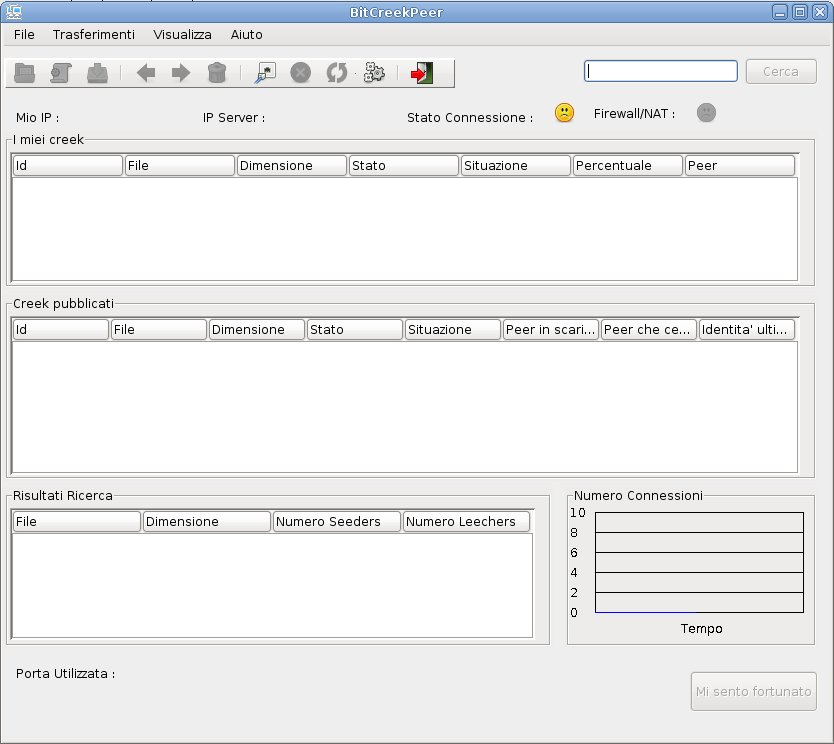
\includegraphics[width=15cm]{images/GUI.jpg}}
  }
  \caption{snapshot della GUI.}
  \label{GUI}
\end{figure}

In questa sezione daremo una spiegazione delle varie politiche e delle scelte implementative fatte, per una descrizione dell'interazione utente-GUI si legga la sezione successiva.
Nella realizzazione della Gui abbiamo posto grande attenzione all'utilizzo delle primitive adeguate per avere un'interfaccia grafica responsiva.
In particolare abbiamo utilizzato i meccanismi della libreria $Javax.Swing$ per la gestione dell'EventQueue, in particolare nessuna delle operazioni invocabili dalla Gui gira sul Thread Dispatcher ma viene assegnato ad un Thread apposito della logica che al termine dell'elaborazione invoca un apposito metodo della Gui per l'aggiornamento della grafica con il metodo $InvokeLater()$.
Con questi meccanismi manteniamo l'interfaccia grafica sempre responsiva anche a seguito di elaborazioni consistenti da parte della logica. In particolare per le funzionalit\`a come la creazione dei Descrittori e la loro ricerca tramite RMI, molto onerose anche a causa dell'interazione client-server, l'interfaccia grafica non presenta freeze. Unica eccezione a questa politica \`e la funzione di connessione, abbiamo infatti ritenuto che nel caso della connessione fosse pi\`u naturale avere un freeze dell'interfaccia fino a che la procedura di connessione al server non \`e completata.
Altro aspetto che abbiamo considerato accuratamente \`e l'abilitazione/disabilitazione dei vari bottoni, evitando quindi che un utente inesperto possa effettuare operazioni prive di senso ed eventualmente dannose per la consistenza dei dati.

\subsubsection{Implementazione della GUI}

La GUI utilizza tre modelli con altrettanti pannelli:
\begin{itemize}
\item modello MieiCreek: visualizza lo stato degli swarm a cui sto partecipando.
\item modello CreekPubblicati: visualizza lo stato degli swarm in cui sono seeder, il peer che ha pubblicato il file ha anche visibilit\`a dei peer che effettuano la ricerca.
\item modello RisultatiRicerca: vengono visualizzati i risultati della ricerca di un file, la ricerca si attiva sia dalla textbox in alto a sinistra che tramite il pulsante "Mi sento fortunato" in basso a destra. Questa funzionalit\`a \`e stata implementata durante il testing dell'applicazione ed \`e rimasta inalterata nella versione finale del progetto.
\end{itemize}

\paragraph{Listener della GUI}
La GUI utilizza due listener, entrambi implementati come SwingTimer. Questi due Thread effettuano una scansione di arrayDescr<Creek> e arrayCercati<Descrittore> nella logica del peer e aggiornano le relative tabelle dell'interfaccia grafica.
In fase di progetto abbiamo deciso di utilizzare i meccanismi degli SwingTimer perch\'e consentono una stesura del codice coerente oltre ad essere preferibile, nel nostro caso, a degli oggetti $Observable$. Degli oggetti $Observable$ avrebbero causato un Overhead eccessivo per il peer e assolutamente ingiustificato. Nel nostro caso abbiamo scelto un delay tra le varie invocazioni del timer di 0.5 secondi nell'aggiornamento delle tabelle e di 1.2 secondi per l'aggiornamento del grafico delle connessioni, la scelta dei valori \`e un buon compromesso tra la responsivit\`a dell'interfaccia grafica e l'overhead introdotto dai Thread.

\subsection{Peer}

Questo Package contiene le varie classi che compongono la logica dell'applicazione e definiscono il protocollo di interazione tra peer.
Al momento dell'avvio (initProtocol) da parte della GUI viene istanziato un oggetto di tipo BitCreekPeer, il suo stato viene ripristinato dalla precendente esecuzione usando dei file di configurazione presenti in una cartella apposita. Come prima cosa l'utente deve connettersi da interfaccia grafica tramite l'apposito tasto, durante la connessione viene invocata la procedura di test del NAT, se la procedura da esito positivo il peer risulta connesso al server. 
A questo punto vengono avviati i vari thread di supporto:
\begin{itemize}
\item Thread KeepAlive
\item Thread Listener
\end{itemize}

%%INSERIRE QUI COMMENTO DELLA SPIEGAZIONE NAT
A questo punto le varie funzionalit\`a della GUI sono attive ed \`e possibile:
\begin{enumerate}
\item creare un nuovo descrittore.
\item creare un file .creek.
\item aprire un file .creek e avviarlo.
\item avviare un file tra quelli cercati.
\item eliminare file (sia in stato di seeder che di leecher).
\item disconnettersi dalla rete.
\item chiudere l'applicazione (ovviamente).
\end{enumerate}

Si osservi il diagramma dei casi d'uso.

\begin{figure}[h]
  \centerline{
    \mbox{\includegraphics[scale=0.8]{images/UseCase.jpg}}
  }
  \caption{Casi d'uso.}
  \label{UseCase}
\end{figure}

\subsubsection{arrayDescr}
Questa classe rappresenta il punto centrale di tutta l'applicazione.
E` implementata come ArrayList$\langle Creek \rangle$ e contiene tutte le informazioni relative ai vari swarm a cui il peer partecipa, ogni singolo oggetto di tipo Creek infatti rappresenta un "Descrittore a runtime" e quindi racchiude tutte le informazioni necessarie a runtime per la gestione di uno swarm. Data la sua importanza riportiamo qui le sue varibili di istanza:

\lstinputlisting[caption=$Creek$.,label=list:Creek]{code/Creek.header}

\subsubsection{Analisi delle varie classi}
Andiamo ad analizzare le varie classi in dettaglio:

Le seguenti classi implementano tramite appositi Thread le funzionalit\`a invocate dalla GUI:
\begin{itemize}
\item Apri
\item Avvia
\item Cerca
\item Crea
\item Riavvia
\end{itemize}

La caratteristica comune di questi Thread \`e di operare principalmente su arraydescr del peer per aggiungere/avviare/eliminare nuovi creek su cui lavorare.
Merita approfondire le operazioni svolte dal thread Avvia in quanto sono significative per comprendere l'avvio di uno scaricamento da parte del peer:
\begin{enumerate}
\item Creazione dell'oggetto creek a partire dal descrittore ricevuto dal server.
\item Controllo di presenza (si verifica che lo swarm non sia gia stato avviato)
\item Settaggio del Creek e aggiunta ad arrayDescr, in questa fase vengono inzializzate tutte le parti del creek NON serializzabili e relative al download, in particolare viene aperto il RandomAccessFile e inizializzata la lista toDo relativa ai chunk da scaricare.
\item Contatto il server in SSL e recupero la listaPeer.
\item Per ogni NetRecord contenuto nella ListaPeer tento una connessione (Handshake applicativo), se ha successo creo un nuovo oggetto Connessione e lo associo ad un Thread Downloader
\item Avvio l'UploadManager
\end{enumerate}

In fase di progetto abbiamo scartato l'ipotesi di introdurre un'ulteriore livello di generalizzazione estendendo la classe Creek in quanto non avrebbe introdotto un ulteriore livello di astrazione ma esclusivamente aggiunto dettagli implementativi alla classe.

%diagramma di sequenza IMPOSSBILE

Questo stesso tipo di interazione \`e riscontrabili in tutti gli altri Thread sopra elencati con lievi differenze, per esempio nel caso di Riavvia i descrittori non vengono selezionati a partire dalla funzionalit\`a di ricerca ma caricati da file system.

\subsubsection{Politiche e Strutture Dati}

A questo punto \`e doveroso dare una panoramica delle politiche e stutture dati utilizzate per la gestione di uno swarm all'interno del peer. La trattazione non pu\`o essere ovviamente esaustiva ma cercheremo di evidenziare i punti salienti della progettazione.
Facciamo notare che ogni swarm viene gestito indipendentemente, l'unica eccezione \`e data dalla gestione del limite connessioni, globale per ogni peer.
Come prima cosa dobbiamo evidenziare che per la realizzazione delle politiche ci siamo attenuti strettamente alle politiche reali di BitTorrent facendo riferimento, quando possibile, al testo \citep{art:rif.1} 
; qualora il testo non fosse risultato di aiuto abbiamo progettato autonomamente le politiche da utilizzare.
In particolare la definizione dei vari messaggi scambiati tra i peer \`e conforme a quella del testo, per la scelta degli algoritmi ci siamo invece attenuti il pi\`u possibile alle politiche di BitTorrent introducendo eventuali modifiche per aumentare le prestazioni.
Come prima cosa \`e utile dare visione delle variabili di istanza dell'oggetto connessione:

\lstinputlisting[caption=$Connessione$.,label=list:Connessione]{code/Connessione.header}

Si nota che l'oggetto connessione wrappa 2 socket, una dedicata al download e una all'upload. Cos\`i facendo abbiamo numerevoli vantaggi. In primo luogo un'astrazione sulle socket vere e proprie che facilita notevolmente la comprensibilit\`a del codice operante sulla connessione. In secondo luogo i Thread Downloader e Uploader che operano sulle connessioni risultano completamente autonomi, l'utilizzo di due socket separate permette ai due thread di operare in maniera totalmente indipendente e con un protocollo a scambio di messaggi semplice e intuitivo. E` risultato a questo punto molto naturale estendere il comportamento del Thread Downloader con le politiche INIT,RAREST e ENDGAME direttamente ricavate dal protocollo BitTorrent.
Diamo una rapido riassunto di queste politiche:
\begin{itemize}
\item INIT: al momento dell'avvio di uno swarm il Chunk da scaricare va scelto in maniera totalmente casuale in maniera da massimizzare la probabilit\`a di ottenere un pezzo utile al pi\`u presto, una volta raggiunto questo obbiettivo si passa in RAREST.
\item RAREST: la scelta dei pezzi avviene in base alla rarit\`a, ad ogni passo il pezzo prescelto \`e quello pi\`u raro, si noti che come politica aggiuntiva abbiamo introdotto una scelta casuale tra pezzi di pari rarit\`a, in un ambiente di test con numero di peer ristretto come quello che avevamo a disposizione (o comunque su swarm poco popolati) l'aumento di prestazioni e distribuzione complessiva del file tra i peer \`e risultata assai maggiore.
\item ENDGAME: al raggiungimento di una soglia specificata ogni singolo Thread effettua una richiesta unica di tutti i pezzi mancanti all'altro peer, l'overhead introdotto da questa tecnica \`e giustificato dall'aumento delle probabilit\`a di completamento di un file con il conseguente rilascio di tutte le risorse occupate dai Thread Downloader (di cui beneficiano anche gli altri peer dato che si aggiunge automaticamente un nuovo seeder).
\end{itemize} L'utilizzo degli oggetti connessione ha inoltre facilitato lo sviluppo del Thread UploadManager, responsabile delle politiche di CHOKE e UNCHOKE; nel realizzarle abbiamo introdotto gli stessi meccanismi utilizzati da BitTorrent con 4 peer UNCHOKE e un peer scelto a caso (OPTIMISTIC UNCHOKE). Nel realizzare le varie politiche abbiamo adottato un approccio coeso realizzando sia la classe Connessione che la classe PIO come implementazione di Comparable, questo ha permesso l'utilizzo dei meccanismi forniti dal package Collections per l'ordinamento:
\begin{itemize}
\item nel caso della politica Rarest utilizzato per ordinare i pezzi da scaricare in base alla rarit\`a.
\item nel caso dell'UploadManager per ordinare le connessioni in base al numero di pezzi scaricati.
\end{itemize}
Si noti a questo punto la bonta della scelta di un oggetto che virtualizzi la connessione: I thread Downloader e Uploader utilizzano metodi e variabili della classe connessione distinti senza introdurre overhead tra di loro dovuto ad eventuali sincronizzazioni. Il thread UplodManager opera interamente sull'oggetto connessione e in basse alle informazioni salvate dal thread Downloader comunica al Thread Uploader il CHOKE o l'UNCHOKE sul pezzo, il tutto per\`o in maniera molto naturale e comprensibile a livello di codice. Se si osserva le operazioni svolte dal Thread UploadManager si nota che esso effettua esclusivamente l'ordinamento della lista Connessioni e le segnalazioni sui Monitor associati.

\subsubsection{Meccanismi di sincronizzazione}

La scelta dei corretti meccanismi di sincronizzazione \`e stata ampiamente ponderata. Per la sincronizzazione tra Thread si \`e fatto uso di metodi synchronized. Come gia specificato precedentemente l'UploadManager fa uso di monitor per gestire gli upload, in questa  maniera abbiamo il duplice vantaggio di una strutturazione del codice elegante e la riduzione dell'overhead dovuta ai Thread Uploader in quanto esclusivamente i thread che posso uploadare sono attivi.
Infine bisogna notare che sono presenti numerosi thread all'interno di BitCreek che operano a intervalli regolari di tempo, per ogni caso \`e stato scelto un meccanismo adeguato allo scopo valutando l'overhead introdotto e i benefici, in particolare.
\begin{itemize}
\item I thread relativi alla GUI, avendo minore priorit\`a rispetto ai thread della logica, utilizzano SwingTimer per andare in esecuzione a intervalli regolari. I motivi di questa scelta sono essenzialmente due: in questa maniera abbiamo una gestione coerente esattamente come se fossere eventi, possiamo utilizzare meccanismi quali InvokeLater per evitare che l'esecuzione di questi thread rallenti l'applicazione. \citep{site:rif.1}
\item I thread quali: sono gestiti come TimerTask in quanto abbiamo ritenuto che un loro eventuale delay nell'esecuzione non costituisse un problema e fosse preferibile un minore overhead.
\item I thread a maggiore priorit\`a infine sono gestiti tramite sleep esplicite in quanto la loro esecuzione a intervalli regolari \`e fondamentale per il corretto funzionamento dell'applicazione o sono necessarri meccanismi di sincronizzazione esplicita come gli interrupt.
\end{itemize}

\subsubsection{Features Aggiuntive: Salva, Terminazione}

Queste due features sono state aggiunte
